\chapter{Analysis}
\label{ch:analysis}
In the analysis
phase, the product requirements are derived --- defining the client expectations
for the product --- as well as the project constraints --- what the environments
limits about the product. Finally, the theoretical foundations are outlined,
providing the basic technical knowledge to undertake the project.
%
  \vspace{-5mm}
%  
\section{Requirements}
\label{sec:requirements}
The requirements defined the client expectations for the TV remote control,
namely:
\begin{item-c}
\item Remotely operated
\item Low weight
\item Powered by batteries
\item 3 buttons: Power (Off/On); Up and Down for channel selection.
\item Infrared emitter response time (system output response time): 100 ms
\item The TV remote may be upgraded in the future to use more buttons
\end{item-c}
%
  \vspace{-5mm}
%  
\section{Constraints}
\label{sec:constraints}
The project constraints are the limitations the environment imposes on it, namely:
\begin{item-c}
\item the TV remote must contain an infrared emitter (the TV already has an infrared receiver)
\item The TV remote control must supply the required data frames imposed by the TV
  manufacturer
\item Data frames may not be provided by the client
\item Security concerns are defined by the data frames and the specific
  communication frequency imposed by the TV manufacturer
\item 1 week deadline: 14 h
\item Manpower: 2 people
\item Budget:
  \begin{itemize}
  \item HW (parts acquisition and assembly): fixed costs --- 1 EUR/unit (1000
    batch production)
    \begin{itemize}
    \item TV remote Shell
    \item TV remote membrane
    \item Data acquisition \& Infrared emitter PCB
    \end{itemize}
  \item Development: project --- 20 EUR per hour per person, totalling 560 EUR +
    IVA
  \end{itemize}
\end{item-c}
%
  \vspace{-5mm}
%  
\section{Theoretical foundations}
\label{sec:theor-found}
The theoretical foundations provide the basic technical knowledge for project
undertaking. In that sense, it is important to understand the principle of
operation and the related technologies, namely the infrared communication
protocol consisting of well-established data frames, specific to each
manufacturer and at specific bandwith. It should be highlighted that the
communication protocol information is critical for the correct behavior of the
TV remote control, as the latter must stimulate the TV, complying to this protocol.

Pushing a button on a remote control sets in motion a series of events
that causes the controlled device to carry out a command. The process
can be generally described as:
\begin{enum-c}
\item 
pushing the button on the remote control causes a touch to the contact beneath it and complete the button circuit on the circuit board. The integrated circuit detects this.
\item 
The integrated circuit sends the binary of the button function command to the
infrared \gls{led} at the front of the remote.
\item 
The \gls{led} emits a series of light pulses that corresponds to the binary the button command.
\end{enum-c}

As an example, one can take a look at the clicking on the ``volume up'' button
on a Sony TV remote (Fig.~\ref{fig:btncode}):
%
  \vspace{-5mm}
%  
%
\begin{figure}[htb!]
\centering
    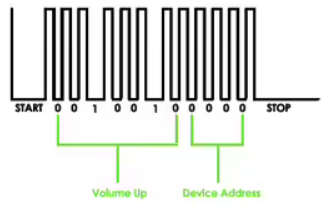
\includegraphics[width=0.45\columnwidth]{./img/buttoncode.png}
  \caption{Example of wave generator for "volume up" from~\cite{btncode}}%
\label{fig:btncode}
\end{figure}

The remote signal includes more than the command for ``volume up''. It sends
several bits of information to the receiving device, establishing a
communication protocol, including:
\begin{item-c}
\item a ``start'' command
\item the command code for ``volume up''
\item the device address (so the TV knows the data is intended for it)
\item a ``stop'' command (triggered when you release the ``volume up'' button)
\end{item-c}

In this case, the buttons that are needed and its codes are:
\begin{item-c}
\item
Power On = 001 0101
\item
Power Off = 010 1111
\item
Volume Up = 001 0010
\item
Volume Down = 001 0011
\end{item-c}
%
  \vspace{-5mm}
%  
\subsection{Reverse engineering}
\label{sec:reverse-engineering}
The contract established between the client (Samsung company) and the developer
team (the authors) imposes the disclosement of the required information about
the communication protocol. However, this is not always necessarily the case. As
such, it is important to have a backup plan, which, in this case, corresponds to
perform reverse engineering on the communication protocol.

For this endeavour, an ``attack'' can be performed on the TV, by stimulating it
at varying frequencies and set of commands and observing its effect. Obviously,
the complexity grows with the number of required commands, but as in this case
there are only 3 commands, this can be feasible. Furthermore, this can be
bootstrapped by using available TV remote control emulators. An example setup
can be connecting an \gls{ir} receiver at a Raspberry Pi, as illustrated in
Fig.~\ref{fig:rasp-lirc} and loading a package, called \gls{lirc} that allows you to decode and send infrared signals of many (but not all) commonly used remote controls.

The most important part of LIRC is the lircd daemon which decodes IR signals
received by the device drivers and provides the information on a socket. It also
accepts commands for IR signals to be sent if the hardware supports
this~\cite{lirc}. Additionally, the sent IR signals can be used to identify the
emitter characteristics, if already present in the database, or simply recorded
for later usage. For the present use case, the list of available commands for
Samsung TVs can also be obtained for the database for actual TV ``attack''.
%
  \vspace{-5mm}
%  
%
\begin{figure}[htb!]
\centering
    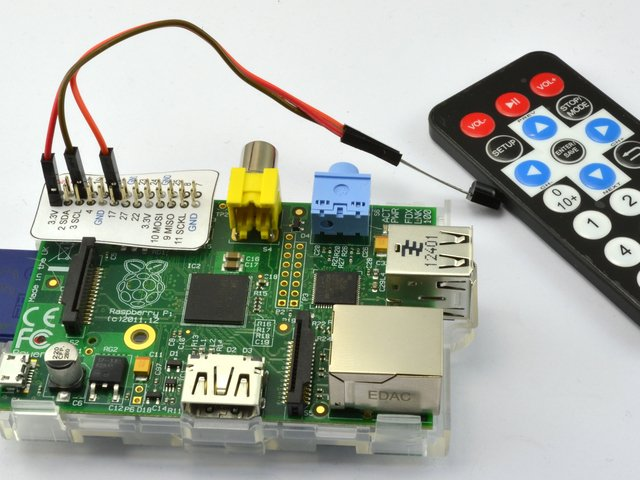
\includegraphics[width=0.43\columnwidth]{./img/rasp-reverse-engineering-setup.jpg}
  \caption{Example setup for reverse engineering of TV remote control commands
    using an emulator~\cite{rasp-lirc}}%
\label{fig:rasp-lirc}
\end{figure}

%%% Local Variables:
%%% mode: latex
%%% TeX-master: "../../dissertation"
%%% End:
